\section{Noise Description}
\label{sec:noise_description}

As mentioned in~\cite{Yahia2013}, there are four main noise sources in the receiver.
In the following each noise source will be described and its transfer function towards the loads will be derived. 
\begin{figure}[h]
\begin{center}
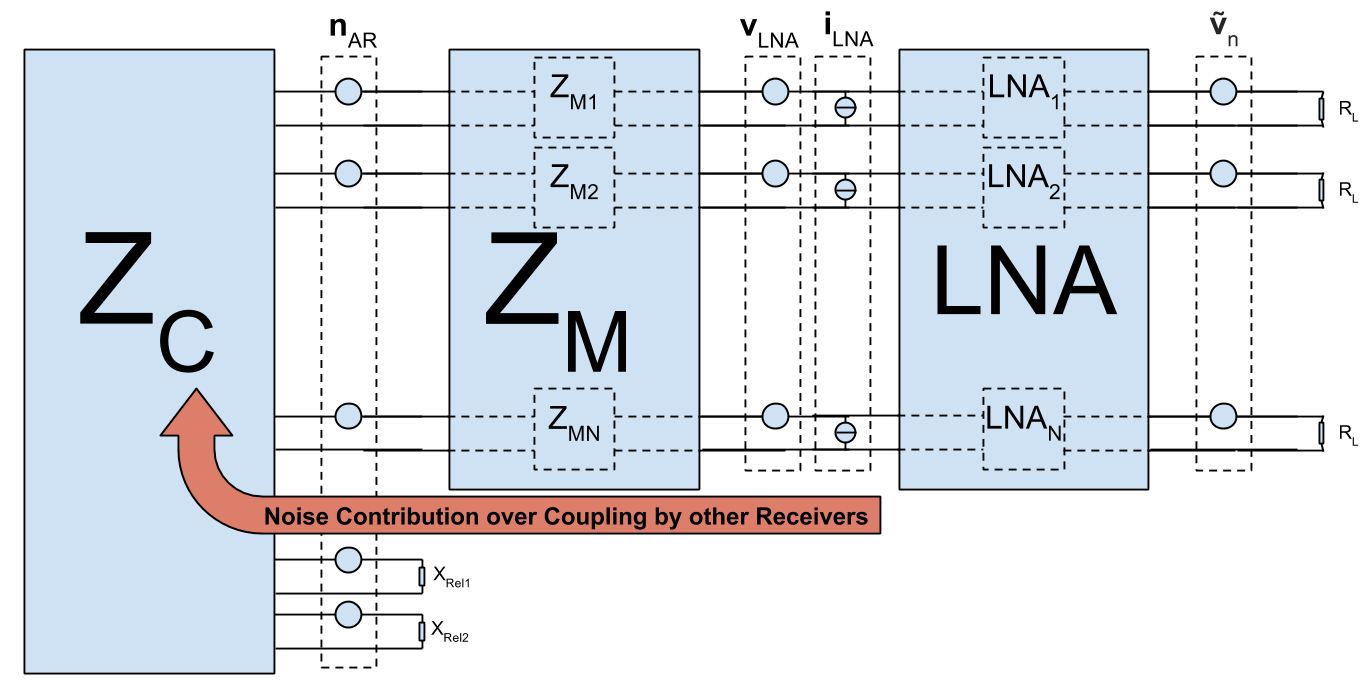
\includegraphics[width=\textwidth]{images/Full_Receiver_noise.png}
\caption{Overview of the system including noise sources.}
\label{fig:receiver_noise}
\end{center}
\end{figure}

Figure~\ref{fig:receiver_noise} gives an overview of the different noise sources.
Important hereby is, that the first three noise sources ($\vec{n}_\text{AR}$, $\vec{v}_\text{LNA}$ and $\vec{i}_\text{LNA}$) also contribute to the other receivers by the coupling.
Only the downstream noise $\vec{\tilde{v}}_n$ is contributing just to its receiver, because of the unilateral assumption of the LNA.

In the following, the transfer functions for the different noise sources will be derived, so that in the end, the total noise contribution at the receiver can be expressed as
\begin{align}\nonumber
\label{eq:noise_contrib}
\vec{u}_\text{L} &= \vec{u}_\text{AR} + \vec{u}_{\text{LNA}_v} + \vec{u}_{\text{LNA}_c} + \vec{u}_{\tilde{n}},\\
&= f(\vec{n}_\text{AR}) + g(\vec{v}_\text{LNA}) + h(\vec{i}_\text{LNA}) + k(\vec{\tilde{v}}_\text{n}),
\end{align}
with $f,g,h,$ and $k$ as the transfer functions for each noise source.

\subsection{Antenna Noise}
\label{sec:antenna_noise}

The antennas introduce two noise sources.
The external noise $\vec{n}_\text{ext}$, collected from the radiation component of the antenna array and the noise generated by the losses in the antennas $\vec{n}_l$.
From~\cite{Twiss1955} it follows, 
\begin{equation}
\label{eq:cov_ant}
\mat{R}_\text{na} = \mathbb{E}[\vec{n}_\text{AR}\vec{n}_\text{AR}^H] = 4 k_B B_W(T_\text{AE}\mathbb{R}\{\mat{Z}_\text{AR}\}+T_\text{AL}\mat{R}_\text{AR}),
\end{equation}
with $k_B$ the Boltzmann constant and $B_W$ the bandwidth.

\subsubsection{Transfer Function of the Antenna Noise}
\label{sec:antenna_noise_transf}
As the antenna noise is picked up by the antennas in the same way as the signal, the transfer function remains the same as the one derived in Equation~\eqref{eq:transfer_function} for the signal, e.g.
\begin{align}
\mat{H}_\text{L,i} &= \mat{H}_\text{L,LNA}\cdot\mat{H}_\text{LNA,M}\cdot\mat{H}_\text{M,O'} \cdot \mat{H}_i^{\text{pr}}.
\end{align}

\subsection{LNA Noise}
\label{sec:lna_noise}

The LNA introduces the third noise source.
From the discussion in~\cite{Nossek}, the noise of the LNA is modeled by a series of voltages and parallel currents at the input of the LNA Block.
The noise sources have the following statistical properties,
\begin{align}
\label{eq:cov_lna}
\mathbb{E}[\vec{i}_\text{LNA}\vec{i}_\text{LNA}^H] &= \beta \cdot \mat{I}_{N_\text{R}N_\text{Rx}},\\\nonumber
\mathbb{E}[\vec{v}_\text{LNA}\vec{v}_\text{LNA}^H] &= \beta \cdot R_n^2\mat{I}_{N_\text{R}N_\text{Rx}},\quad\text{and}\\\nonumber
\mathbb{E}[\vec{v}_\text{LNA}\vec{i}_\text{LNA}^H] &= \rho \beta \cdot R_n\mat{I}_{N_\text{R}N_\text{Rx}},
\end{align}
with $\rho$ and $\beta$ as correlation coefficients.

\subsubsection{Transfer Function of the LNA Noise}
\label{sec:antenna_noise_transf}
As written above, we have two noise sources, the serial voltage sources and the parallel current sources.
For both of them, we need to consider, that at the loads, we have noise contribution of the LNA of the own receiver branch and LNA noise of the other receiver branches, by the coupling.
Therefore two transfer functions will be derived in the following:
\begin{enumerate}
\item The indirect - a transfer function towards the antenna, and
\item The direct - a transfer function towards the loads.
\end{enumerate}
With the indirect transfer function derived, we can (as in the previous section) concatenate the transfer function of the signal, to get the LNA noise contribution of the other receivers. 

\paragraph{Direct LNA Noise Contribution:}
First we will transfer the current source into a voltage source in series as we then can use the same transfer function for the voltage and the transferred current sources.
To do so, we need the equivalent input impedances looking from the left into the LNA block and from the right into the matching network.
The equivalent input impedance for the LNA network $\mat{Z}_{\text{eqLNA}_1}$ was already derived in~\eqref{eq:zeqlna1}.
To get the equivalent input impedance for the matching network looking from the right into it we use Equation~\eqref{eq:eq_imp_load} and get
\begin{align}
\label{eq:zr}
\mat{\tilde{Z}}_{\text{eqM}_2} &= \mat{Z}_\text{M22} - \mat{Z}_\text{M12}\cdot(\mat{Z}_\text{M11} + \mat{Z}_\text{C'})^{-1}\cdot\mat{Z}_\text{M21}.
\end{align}

Transferring the current source into a series of voltages gives us 
\begin{equation}
\vec{v}_{\text{LNA}_c} = -\mat{\tilde{Z}}_{\text{eqM}_2} \vec{i}_\text{LNA},
\end{equation}

and therefore a transfer function of
\begin{equation}
\label{eq:lnavdir}
\mat{H}_\text{L,LNAv,dir} = R_\text{L}\mat{I}_{N_R}(R_\text{L}\mat{I}_{N_R} + \mat{\tilde{Z}}_{\text{eqLNA}_2})^{-1}\mat{e}\cdot(\mat{c}+\mat{\tilde{Z}}_{\text{eqM}_2})^{-1},
\end{equation}
for the series voltages and
\begin{align}\nonumber
\label{eq:lnacdir}
\mat{H}_\text{L,LNAc,dir} &= -R_\text{L}\mat{I}_{N_R}(R_\text{L}\mat{I}_{N_R} + \mat{\tilde{Z}}_{\text{eqLNA}_2})^{-1}\mat{e}\cdot(\mat{c}+\mat{\tilde{Z}}_{\text{eqM}_2})^{-1}\mat{\tilde{Z}}_{\text{eqM}_2},\\
 &= - \mat{H}_\text{L,LNAv,dir}\cdot \mat{\tilde{Z}}_{\text{eqM}_2},
\end{align}
for the LNA noise currents.
Both transfer functions assume user $i$ to be the receiver.
It is clear to see, that both transfer functions are of size $\mathbb{C}^{N_\text{Rx}\times N_\text{Rx}}$

\paragraph{Indirect LNA Noise Contribution:}
In a second step we transfer the LNA-voltage and -current sources, respectively to parallel voltage sources at the antennas, so that the transfer function derived in Equation~\eqref{eq:transf_func} can be applied.
In the following, all the indices are neglected for simplicity reasons.
For the transfer functions towards the antennas, we consider all the ports of the passive receivers.
Therefore we are looking at matrices of size $\mathbb{C}^{(N_\text{R}-1)N_\text{Rx}\times (N_\text{R}-1)N_\text{Rx}}$.

By multiplying the LNA-current noise source by the equivalent input impedance of the LNA
\begin{align}
\vec{v}_\text{LNAc} = \mat{Z}_{\text{eqLNA1}} \vec{i}_\text{LNA},
\end{align}
it is transferred to a series voltage, just like the LNA-voltage noise.
Now we only need to find the transfer function for the LNA-voltage source $\vec{v}_\text{LNAv}$.
The transfer function over the matching network is given by
\begin{align}
\label{eq:lnanoise_to_input}
\mat{H}_\text{O,LNA} = \mat{Z}_\text{M12}(\mat{Z}_\text{M22}+\mat{Z}_{\text{eqLNA1}})^{-1}.
\end{align}
This leads to the overall indirect LNA noise transfer functions of
\begin{align}
\label{eq:lnaind}\nonumber
\mat{H}_\text{L,LNAv,ind} &= \mat{H}_\text{L,i}\cdot\mat{H}_\text{O,LNA},\quad\text{for the voltage sources, and}\\
\mat{H}_\text{L,LNAc,ind} &= \mat{H}_\text{L,LNAv,ind}\cdot\mat{Z}_{\text{eqLNA1}},\quad\text{for the current sources}.
\end{align}
Looking at the size of the matrices, we see, that the $\mat{H}_\text{O,LNA}$ as well as $\mat{Z}_{\text{eqLNA1}}$ are of size $\mathbb{C}^{(N_\text{R}-1)N_\text{Rx}\times (N_\text{R}-1)N_\text{Rx}}$ and therefore the overall transfer function is of size $\mathbb{C}^{N_\text{Rx}\times (N_\text{R}-1)N_\text{Rx}}$.

\subsection{Downstream Noise}
\label{sec:down_noise}
The last noise source is the downstream noise, generated by all the circuitry after the LNA~\cite{Hughes2012} and modeled by voltage sources $\vec{\tilde{v}}_\text{n}$ in series to the loads.
With the statistical property
\begin{equation}
\label{eq:cov_down}
\mathbb{E}[\vec{\tilde{v}}_\text{n}\vec{\tilde{v}}_\text{n}^H] = \psi\cdot\mat{I}_{N_\text{R}N_\text{Rx}}.
\end{equation}

\subsubsection{Transfer Function of the Downstream Noise}
\label{sec:down_noise_transf}
For the transfer function of the downstream noise we need a simple voltage divider of the loads and the equivalent input impedance $\mat{\tilde{Z}}_{\text{eqLNA}_2}$ looking from the right into the LNA block.
\begin{equation}
\label{eq:down_tf}
\mat{H}_\text{L,n} = R_\text{L}\mat{I}_{N_R}(R_\text{L}\mat{I}_{N_R} + \mat{\tilde{Z}}_{\text{eqLNA}_2})^{-1},
\end{equation}
with 
\begin{align}
\label{eq:zeqlna2_down}
\mat{\tilde{Z}}_{\text{eqLNA}_2} &= \mat{g} - \mat{d}\cdot(\mat{c} + \mat{\tilde{Z}}_{\text{eqM}_2})^{-1}\cdot\mat{e} = \mat{g},
\end{align}
whereby the unilateral assumption ($\vec{d}=\mat{0}$) was applied, and hence $\mat{\tilde{Z}}_{\text{eqLNA}_2}=\mat{Z}_{\text{eqLNA}_2}$ from Equation~\eqref{eq:zeqlna2}.

For the downstream noise we note, that under the unilateral assumption, the transferred noise towards the antennas is zero, because
\begin{align}
\vec{v}_\text{LNAn} = \mat{d}(\mat{g}+R_\text{L}\mat{I}_{N_R})^{-1} \tilde{\vec{v}}_{v}=0,
\end{align}
when $\mat{d}=0$.
Therefore, the downstream noise does only contribute to its own receiver branch, and hence $\mat{H}_\text{L,n}$ is of size $\mathbb{C}^{N_\text{Rx}\times N_\text{Rx}}$.

\subsection{Noise Covariance Matrix}
\label{sec:sig_cov}
In the following we will describe the whole system by its noise transfer functions.
We thereby use the index $i$ for the branches of the active receivers and index $j$ for the branches of the passive receiver, i.e. the branches which contributed only by their coupling.
With the transfer functions derived for each noise source, we can finally express each noise contribution at the loads as stated in Equation~\eqref{eq:noise_contrib} by
\begin{align}
\label{eq:noise_output}
\nonumber
\vec{u}_\text{AR} &= \mat{H}_\text{L,0}\cdot\vec{n}_\text{AR},\\\nonumber 
\vec{u}_{\text{LNA}_v} &= 
	\mat{H}_\text{L,LNAv,ind}\cdot\vec{v}_{\text{LNA},j}+
	\mat{H}_\text{L,LNAv,dir}\cdot\vec{v}_{\text{LNA},i},\\\nonumber
\vec{u}_{\text{LNA}_c} &= 
	\mat{H}_\text{L,LNAc,ind}\cdot\vec{i}_{\text{LNA},j}+
	\mat{H}_\text{L,LNAc,dir}\cdot\vec{i}_{\text{LNA},i},\\\nonumber
\vec{u}_{\tilde{n}} &= \mat{H}_\text{L,n}\cdot\vec{\tilde{v}}_{n},\\
\text{and therefore}\qquad &\vec{u}_\text{L} = \vec{u}_\text{AR} + \vec{u}_{\text{LNA}_v} + \vec{u}_{\text{LNA}_c} + \vec{u}_{\tilde{n}}.
\end{align}

As each vector is of size $\mathbb{C}^{ N_\text{Rx}\times 1}$, the noise covariance matrix, described in the following will be of size $\mathbb{C}^{ N_\text{Rx}\times N_\text{Rx}}$.
Because all the noise sources are uncorrelated, except for the LNA noise sources (c.f. Equation~\eqref{eq:cov_lna}), the noice covariance matrix can be written as:
\begin{align}
\label{eq:exp_noise}\nonumber
\mat{K}_{\text{N,}i} =\mathbb{E}[\vec{u}_\text{L}\vec{u}_\text{L}^H] &=
\mathbb{E}[\vec{u}_\text{AR}\vec{u}_\text{AR}^H]+ 
\mathbb{E}[\vec{u}_{\text{LNA}_v}\vec{u}_{\text{LNA}_v}^H] +
\mathbb{E}[\vec{u}_{\text{LNA}_v}\vec{u}_{\text{LNA}_c}^H] +\\%\nonumber
\quad&\mathbb{E}[\vec{u}_{\text{LNA}_c}\vec{u}_{\text{LNA}_v}^H] +
\mathbb{E}[\vec{u}_{\text{LNA}_c}\vec{u}_{\text{LNA}_c}^H] +
\mathbb{E}[\vec{u}_{\tilde{n}}\vec{u}_{\tilde{n}}^H].
%\mat{K}_{\text{N,}i} =\mathbb{E}[\vec{u}_\text{L}\vec{u}_\text{L}^H] = &\mat{H}_\text{L,i}\mathbb{E}[\vec{n}_\text{AR}\vec{n}_\text{AR}^H]\mat{H}_\text{L,i}^H + 
%\mathbb{E}[\vec{u}_{\text{LNA}_v}\vec{u}_{\text{LNA}_v}^H] +
%\mathbb{E}[\vec{u}_{\text{LNA}_v}\vec{u}_{\text{LNA}_c}^H] +\\%\nonumber
%\quad&\mathbb{E}[\vec{u}_{\text{LNA}_c}\vec{u}_{\text{LNA}_v}^H] +
%\mathbb{E}[\vec{u}_{\text{LNA}_c}\vec{u}_{\text{LNA}_c}^H] +
%\mathbb{E}[\vec{u}_{\tilde{n}}\vec{u}_{\tilde{n}}^H].
\end{align}

For simplicity reasons, we will look in every summand separately in the following.
For the antenna noise it follows therefore
\begin{align}
\mathbb{E}[\vec{u}_\text{AR}\vec{u}_\text{AR}^H] = 
	\mat{H}_\text{L,i}\mathbb{E}[\vec{n}_\text{AR}\vec{n}_\text{AR}^H]\mat{H}_\text{L,i}^H 
	= \mat{H}_\text{L,i} \mat{R}_\text{na} \mat{H}_\text{L,i}^H,
\end{align}
using~\eqref{eq:cov_ant}, with $\mat{R}_\text{na}$ of size $\mathbb{R}^{ N_\text{R}\cdot\left(N_\text{Rx}+N_\text{Rel}\right)\times N_\text{R}\cdot\left(N_\text{Rx}+N_\text{Rel}\right)}$ and hence, by the shape of $\mat{H}_\text{L,i}$, $\mathbb{E}[\vec{u}_\text{AR}\vec{u}_\text{AR}^H]$ becomes a matrix of size $\mathbb{C}^{ N_\text{Rx}\times N_\text{Rx}}$.


For the LNA voltage noise, using~\eqref{eq:cov_lna}, it follows
\begin{align}
\nonumber
\mathbb{E}[\vec{u}_{\text{LNA}_v}\vec{u}_{\text{LNA}_v}^H] &= 
\mathbb{E}[\left(\mat{H}_\text{L,LNAv,ind}\cdot\vec{v}_{\text{LNA},j}+\mat{H}_\text{L,LNAv,dir}\cdot\vec{v}_{\text{LNA},i}\right)\cdot\\
&\qquad\left(\mat{H}_\text{L,LNAv,ind}\cdot\vec{v}_{\text{LNA},j}+\mat{H}_\text{L,LNAv,dir}\cdot\vec{v}_{\text{LNA},i}\right)^H],
\end{align}
by the fact, that $\vec{v}_{\text{LNA},j}$ and $\vec{v}_{\text{LNA},i}$ are independent of each other (c.f. Equation~\eqref{eq:cov_lna}), the cross terms cancel out an hence,
\begin{align}
\nonumber
\mathbb{E}[\vec{u}_{\text{LNA}_v}\vec{u}_{\text{LNA}_v}^H]&=
	\mat{H}_\text{L,LNAv,ind}\cdot
	\mathbb{E}[\vec{v}_{\text{LNA},j}\vec{v}_{\text{LNA},j}^H]\cdot
	\mat{H}_\text{L,LNAv,ind}^H+\\\nonumber
&\qquad \mat{H}_\text{L,LNAv,dir}\cdot
	\mathbb{E}[\vec{v}_{\text{LNA},i}\vec{v}_{\text{LNA},i}^H]\cdot
	\mat{H}_\text{L,LNAv,dir}^H\\
&=\left(\mat{H}_\text{L,LNAv,ind}\cdot\mat{H}_\text{L,LNAv,ind}^H+
	\mat{H}_\text{L,LNAv,dir}\cdot\mat{H}_\text{L,LNAv,dir}^H\right)\cdot \beta \cdot R_n^2.
\end{align}
for the LNA-voltage source and similar for the current source
\begin{align}
\mathbb{E}[\vec{u}_{\text{LNA}_c}\vec{u}_{\text{LNA}_c}^H]&= 
\left(\mat{H}_\text{L,LNAc,ind}\cdot\mat{H}_\text{L,LNAc,ind}^H+
	\mat{H}_\text{L,LNAc,dir}\cdot\mat{H}_\text{L,LNAc,dir}^H\right)\cdot \beta.
\end{align}

The remaining terms for the LNA noise contribution are the cross terms.
For them it follows,
\begin{align}
\nonumber
\mathbb{E}[\vec{u}_{\text{LNA}_c}\vec{u}_{\text{LNA}_v}^H] +&
\mathbb{E}[\vec{u}_{\text{LNA}_c}\vec{u}_{\text{LNA}_c}^H] = 
	\mat{H}_\text{L,LNAv,dir} 
	\cdot\rho\beta \cdot R_n \cdot
	\mat{H}_\text{L,LNAc,dir}^H +\\\nonumber
&\quad	\mat{H}_\text{L,LNAc,dir} 
	\cdot\rho^*\beta \cdot R_n \cdot
	\mat{H}_\text{L,LNAv,dir}^H +\\\nonumber
&\quad	\mat{H}_\text{L,0}\cdot\mat{H}_\text{L,LNAv,ind} 
	\cdot\rho\beta \cdot R_n \cdot
	\mat{H}_\text{L,LNAc,ind}^H\mat{H}_\text{L,0}^H + \\\nonumber
&\quad	\mat{H}_\text{L,0}\cdot\mat{H}_\text{L,LNAc,ind} 
	\cdot\rho^*\beta \cdot R_n \cdot
	\mat{H}_\text{L,LNAv,ind}^H\mat{H}_\text{L,0}^H\\\nonumber
&= \beta \cdot R_n\biggl(
	-\mat{H}_\text{L,LNAv,dir} \left(\rho\mat{\tilde{Z}}_{\text{eqM}_2}^H+
	\mat{\tilde{Z}}_{\text{eqM}_2}\rho^*\right) \mat{H}_\text{L,LNAv,dir}+\\\nonumber
&\quad	\mat{H}_\text{L,LNAv,ind} \left(\rho\mat{Z}_{\text{eqLNA}_1}^H+
	\mat{Z}_{\text{eqLNA}_1}\rho^*\right) \mat{H}_\text{L,LNAv,ind}\biggr)\\\nonumber
&= 2\beta \cdot R_n\biggl(
	-\mat{H}_\text{L,LNAv,dir} \cdot\mathbb{R}\{\rho^*\mat{\tilde{Z}}_{\text{eqM}_2}\}\cdot
	\mat{H}_\text{L,LNAv,dir}+\\
&\quad	\mat{H}_\text{L,LNAv,ind} \cdot\mathbb{R}\{\rho^*\mat{Z}_{\text{eqLNA}_1}\}\cdot
	\mat{H}_\text{L,LNAv,ind}\biggr),
\end{align}
where Equations~\eqref{eq:cov_lna},~\eqref{eq:lnacdir} and~\eqref{eq:lnaind} where used.

Finally, there is only the downstream noise contribution left.
Because of the unilateral assumption, this becomes less complex, i.e.
\begin{align}
\nonumber
\mathbb{E}[\vec{u}_{\tilde{n}}\vec{u}_{\tilde{n}}^H]&=
\psi\left(\mat{H}_\text{L,n}\cdot\mat{H}_\text{L,n}^H\right),
\end{align}
where the statistical property of the downstream noise from Equation~\eqref{eq:cov_down} was used.

With these results we can form the final noise covariance matrix as 
\begin{align}
\label{eq:noise_cov}\nonumber
\mat{K}_{\text{N},i}%&= 
%	\mathbb{E}[\vec{u}_\text{AR}\vec{u}_\text{AR}^H]+
%	\mathbb{E}[\vec{u}_{\text{LNA}_v}\vec{u}_{\text{LNA}_v}^H]+
%	\mathbb{E}[\vec{u}_{\text{LNA}_c}\vec{u}_{\text{LNA}_c}^H]+\\\nonumber
%&\quad	\mathbb{E}[\vec{u}_{\text{LNA}_c}\vec{u}_{\text{LNA}_v}^H] +
%	\mathbb{E}[\vec{u}_{\text{LNA}_c}\vec{u}_{\text{LNA}_c}^H] +
%	\mathbb{E}[\vec{u}_{\tilde{n}}\vec{u}_{\tilde{n}}^H]\\\nonumber
&=\mat{H}_\text{L,i} \mat{R}_\text{na} \mat{H}_\text{L,i}^H+\\\nonumber
&\quad	\beta \cdot R_n^2\cdot \left(\mat{H}_\text{L,LNAv,ind}\cdot\mat{H}_\text{L,LNAv,ind}^H+
	\mat{H}_\text{L,LNAv,dir}\cdot\mat{H}_\text{L,LNAv,dir}^H\right)+\\\nonumber
&\quad	\beta \cdot \left(\mat{H}_\text{L,LNAc,ind}\cdot\mat{H}_\text{L,LNAc,ind}^H+
	\mat{H}_\text{L,LNAc,dir}\cdot\mat{H}_\text{L,LNAc,dir}^H\right)+\\\nonumber
&\quad	2\beta \cdot R_n\biggl(
	-\mat{H}_\text{L,LNAv,dir} \cdot\mathbb{R}\{\rho^*\mat{\tilde{Z}}_{\text{eqM}_2}\}\cdot
	\mat{H}_\text{L,LNAv,dir}+\\\nonumber
&\quad	\mat{H}_\text{L,LNAv,ind} \cdot\mathbb{R}\{\rho^*\mat{Z}_{\text{eqLNA}_1}\}\cdot
	\mat{H}_\text{L,LNAv,ind}\biggr)+\\
&\quad	\psi\left(\mat{H}_\text{L,n}\cdot\mat{H}_\text{L,n}^H\right).
\end{align}
According to the noise vector sizes given in the beginning of this section, the noise covariance matrix is of size $\mathbb{C}^{N_\text{Rx}\times N_\text{Rx}}$.









